\documentclass[10pt,a4paper,notitlepage]{article}
\usepackage[utf8]{inputenc}
\usepackage{amsmath}
\usepackage{amsfonts}
\usepackage{amssymb}
\usepackage{graphicx}
\title{Crosstalk measurements from PAPER}
\author{Saul A. Kohn$^1$\thanks{saulkohn@sas.upenn.edu}\,\,\,, James E. Aguirre$^1$ \,\,\,\& Ridhima Nunhokee$^{1,2}$\\
$^1$\small{University of Pennsylvania}\\
$^2$\small{Rhodes University} }
\begin{document}
\maketitle

\abstract{Crosstalk is artificial signal created by an interferometer that contaminates the astronomical visibilities it is built to measure.  In this memo, we describe measurements of crosstalk in data from PAPER-64. We present extremely compelling evidence that the dominant source of crosstalk for PAPER is reflections between antenna pairs, demonstrating a $1/R^2$ dependence for antenna-separation $R$. Some crosstalk is seen in excess of this trend, and may be due to crosstalk between dipole arms on individual antennae. We provide the first imaging-based measurements of dipole-arm crosstalk using images from the PAPER-32 imaging configuration. A natural extension of this work is a full modelling of reflections throughout the array, and a more detailed, visibility-based analysis of leakage between dipole arms.}

\section{Introduction \& Theory}
\label{sec:intro}
XXX brief introduction and definitions\\

\subsection{Reflection crosstalk}
\label{subsec:theory_reflection}
We can describe crosstalk from reflections between antenna pair ($m,n$) as:
\begin{equation}
X'_m = X_m + \epsilon^x_{mn}X_n + \epsilon^y_{mn}Y_n;~~~~\epsilon^p_{mn}\propto\frac{1}{|m-n|^2}
\end{equation}
\noindent with a similar definition for $Y_m$; $|m-n|$ represents the physical distance between antennae $m$ and $n$.

This means that the observed $XX$ visibility between antennae becomes:
\begin{equation}
X'_mX'_n = X_mX_n + \epsilon^x_{nm}X_mX_m + \epsilon^x_{mn}X_nX_n + \epsilon^y_{nm}X_mY_m + \epsilon^y_{mn}Y_nX_n + \mathcal{O}(\epsilon^2)
\end{equation}
\noindent However the $XY$ visibilities are noise-like, so effectively:
\begin{equation}
X'_mX'_n \approx X_mX_n + \epsilon^x_{nm}X_mX_m + \epsilon^x_{mn}X_nX_n 
\end{equation}
\noindent Implying that the observed $XX$ visibilities are contaminated by over-the-air crosstalk from autocorrelations of nearby antennae.

\subsection{Dipole-arm crosstalk}
\label{subsec:theory_dterms}
Crosstalk between dipole arms on a given antenna $m$ can be described by (neglecting noise terms):
\begin{align*}
X'_m = X_m + D^x_mY_m\\
Y'_m = Y_m + D^y_mX_m
\end{align*}
\noindent So an observed $XX$ visibility becomes contaminated by noise-like $XY$ and $YX$ visibilities:
\begin{equation}
X'_mX'_n = X_mX_n + D^x_mY_mX_n + D^x_nX_mY_n  + \mathcal{O}(D^2)
\end{equation}
\noindent Which is negligible compared to the $XX$ signal. However, this \textit{polarized leakage} is symmetric, causing $XX$ to leak into $XY$:
\begin{equation}
X'_mY'_n=X_mY_n + D^x_mY_mY_n + D^y_mX_nX_m + \mathcal{O}(D^2)
\end{equation}
\noindent This demonstrates the importance of trying to remove crosstalk when making measurements of polarization -- they will be completely overpowered by the $XX$ and $YY$ terms otherwise.

\subsection{Putting it together}
\label{subsec:theory_both}
Using these models, we can represent crosstalk on a given dipole arm as:
\begin{equation}
\begin{bmatrix}
X'_m\\
Y'_m\\
\end{bmatrix}
=
\begin{bmatrix}
1 & D^x_m \\
D^y_m & 1 \\
\end{bmatrix}
\begin{bmatrix}
X_m\\
Y_m\\
\end{bmatrix}
+
\begin{bmatrix}
\epsilon^{xx}_{mn} &\epsilon^{xy}_{mn} \\
\epsilon^{yx}_{mn} &\epsilon^{yy}_{mn} \\
\end{bmatrix}
\begin{bmatrix}
X_n\\
Y_n\\
\end{bmatrix}
\end{equation} 

\noindent We can represent this in a more condensed form as:
\begin{equation}
\vec{m}' = \boldsymbol{D_m}\vec{m} + \boldsymbol{E_{mn}}\vec{n}
\end{equation}
\noindent Such that:
\begin{equation}
\vec{m}'\otimes\vec{n}'
=
\begin{bmatrix}
X_mXn & X_mY_n \\
Y_mX_n & Y_mY_n\\
\end{bmatrix}
=
(\boldsymbol{D_m}\vec{m} \otimes \boldsymbol{D_n}\vec{n})
+
(\boldsymbol{D_m}\vec{m} \otimes \boldsymbol{E_{nm}}\vec{m})
+
(\boldsymbol{E_{mn}}\vec{n} \otimes \boldsymbol{D_n}\vec{n})
+
(\boldsymbol{E_{mn}}\vec{n} \otimes \boldsymbol{E_{nm}}\vec{m})
\end{equation}


\section{Method}
\label{sec:method}

\subsection{Measuring crosstalk}
\label{subsec:method_xtalk}
We model reflection crosstalk as if it is constant over time. As shown above, this is not quite true, since the amount of reflection crosstalk is proportional to the autocorrelations, and these in turn are proportional to sky temperature. However, a constant over time is usually a good approximation, especially for the large amount of the season in which the Galaxy is not transiting zenith during observations.

Using this constant-over-time model, we proceed with a number of steps to constrain the crosstalk signal based on time-averaged visibilities, extracting the average:
\begin{itemize}
\item  visibility for each baseline, over a 10 minute observation
\item  visibility for each baseline, over a night of observations
\item  visibility for each baseline type over a night of observations
\end{itemize}
\noindent where ``baseline type" refers to a given antenna separation within the PAPER-64 grid. In this case, crosstalk removal is simply a subtraction of the nightly average for each baseline. For analysis of reflection crosstalk we focus on fiducial night JD2456250 from early in the PAPER-64 season, analysing the visibilities between LST=0--8 hours, after sunset. This night has comparable crosstalk levels to other nights in the season, and presents small deviations ($<3\sigma$) from the median sky model at the central frequency of 145\,MHz. 

\subsection{Measuring dipole-arm leakage}
\label{subsec:method_dterms}
The leakage between dipole arms is not configuration dependent. Under the assumption of identical feeds, we can proceed with an imaging-based calibration of the leakage terms using the PAPER-32 polarized imaging configuration following Equations~(4.63) and (4.64) of \cite{TMS}. Assuming Pictor A to be an unpolarized point source, we can make observed $I'$, $Q'$, $U'$ and $V'$ Stokes images of the source at different times, weighting by the beam appropriately.  

It follows that the parameters:

\begin{equation}
\delta_{+-} = D^x_m - D^y_m + D^x*_n - D^y*_n = 2\frac{U'}{I'}
\end{equation}

\begin{equation}
\delta_{-+} = D^x_m + D^y_m - D^x*_n - D^y*_n = -2\frac{V'}{I'}
\end{equation}

\noindent Which allows us to least-squares solve for the $D$-terms with three observations of the unpolarized source using the formulation:

\begin{equation}
\begin{bmatrix}
\delta_{+-,1} \\
\delta_{-+,1} \\
\delta_{+-,2} \\
\delta_{-+,2} \\
\delta_{+-,3} \\
\delta_{-+,3} \\
\end{bmatrix}
=
\begin{bmatrix}
1 & -1 & 1 & -1 \\
1 & 1 & -1 & -1 \\
1 & -1 & 1 & -1 \\
1 & 1 & -1 & -1 \\
1 & -1 & 1 & -1 \\
1 & 1 & -1 & -1 \\
\end{bmatrix}
\begin{bmatrix}
D_{xm}\\
D_{ym}\\
D*_{xn}\\
D*_{yn}\\
\end{bmatrix}
\end{equation}

\section{Results}
\label{sec:results}
In this section we will show the steps outlined in the section above, and our interpretation of... XXX\\

ALL FOR NIGHT 2456250\\

CROSSTALK DIVIDED BY RMS OF VISIBILITY

\begin{figure}
\centering
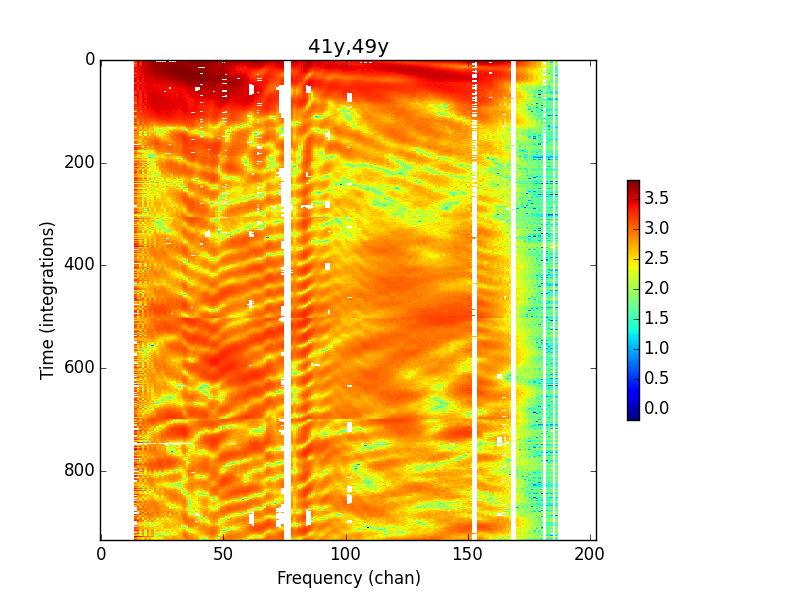
\includegraphics[width=0.4\textwidth]{6250_C.png}
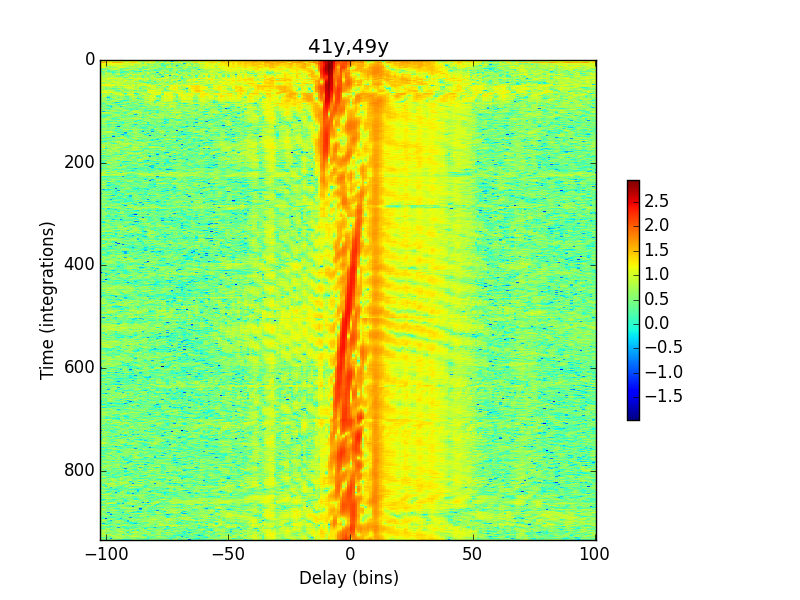
\includegraphics[width=0.4\textwidth]{6250_C_d.png}
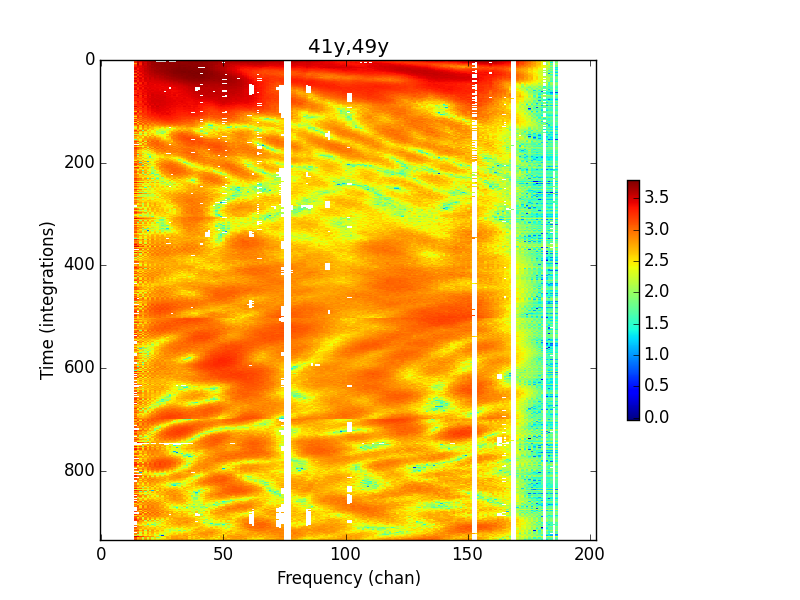
\includegraphics[width=0.4\textwidth]{6250_Cx.png}
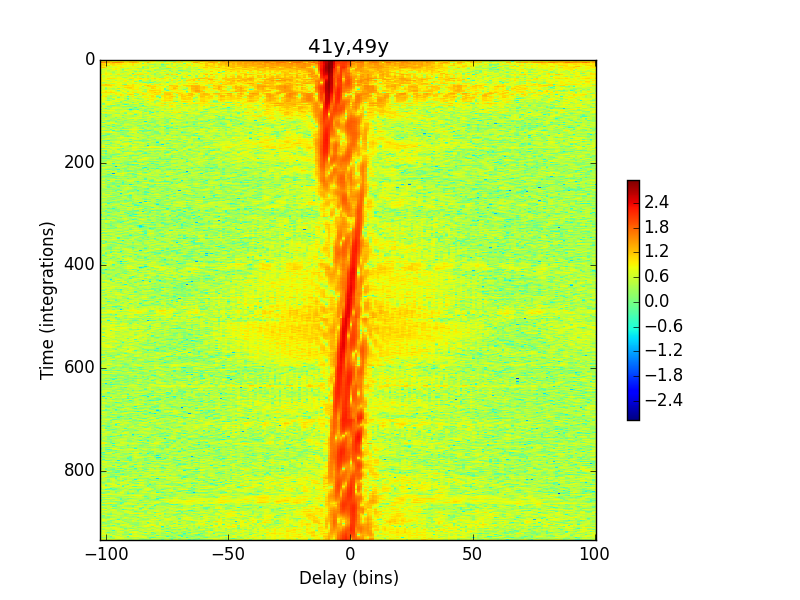
\includegraphics[width=0.4\textwidth]{6250_Cx_d.png}
\caption{\textit{Top}: Waterfall plots of the real part of $YY$ visibilities on a 30\,m baseline in frequency- (left) and delay-space (right). Note the constant-in-time signal on the horizon at positive delay. \textit{Bottom}: the same as above, but after crosstalk subtraction. The bright excess at integration numbers $<$200 is solar. These visibilities have not been CLEANed, leading to noticeable leakage outside of the horizon in delay space.}
\label{fig:waterfalls}
\end{figure}

\begin{figure}
\centering
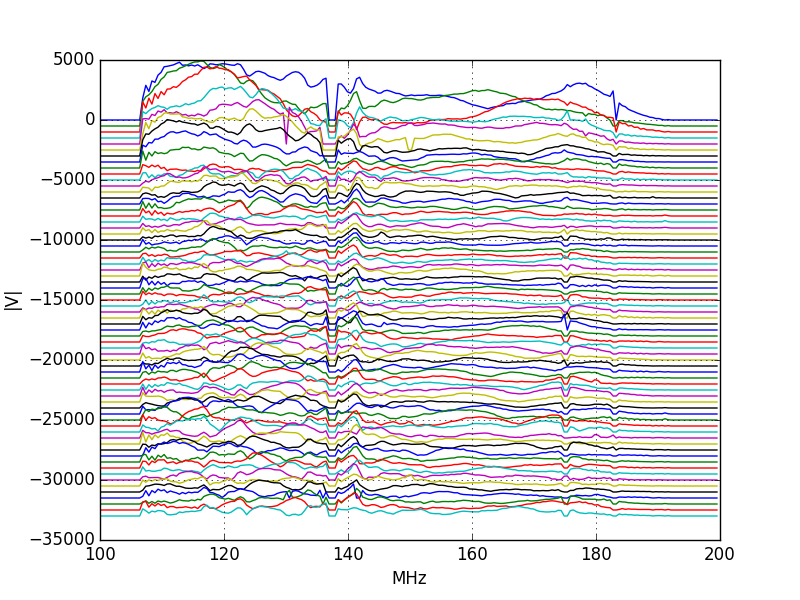
\includegraphics[width=0.4\textwidth]{6250_yy_xtalk_per_file.png}
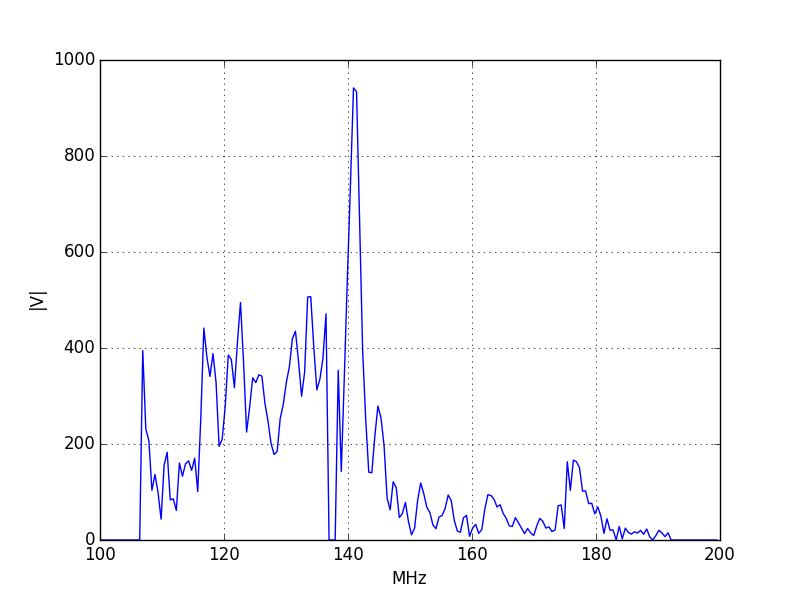
\includegraphics[width=0.4\textwidth]{6250_yy_xtalk_that_night.png}
\caption{\textit{Left}: The average $YY$ visibility for a 30\,m baseline of each 10 minute file over the night, plus a constant offset for display purposes. The average of the first file is at the top, and file time progresses downwards. \textit{Right}: The average of these signals (i.e. average for the night).}
\label{fig:xtalk-per-file}
\end{figure}

\begin{figure}
\centering
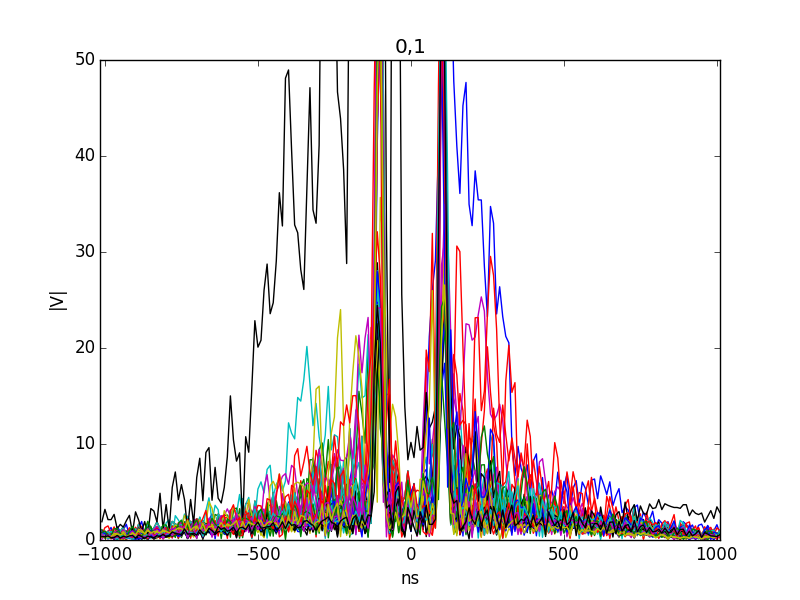
\includegraphics[width=0.4\textwidth]{6250_yy_xtalk_that_night_BLtype1_d.png}
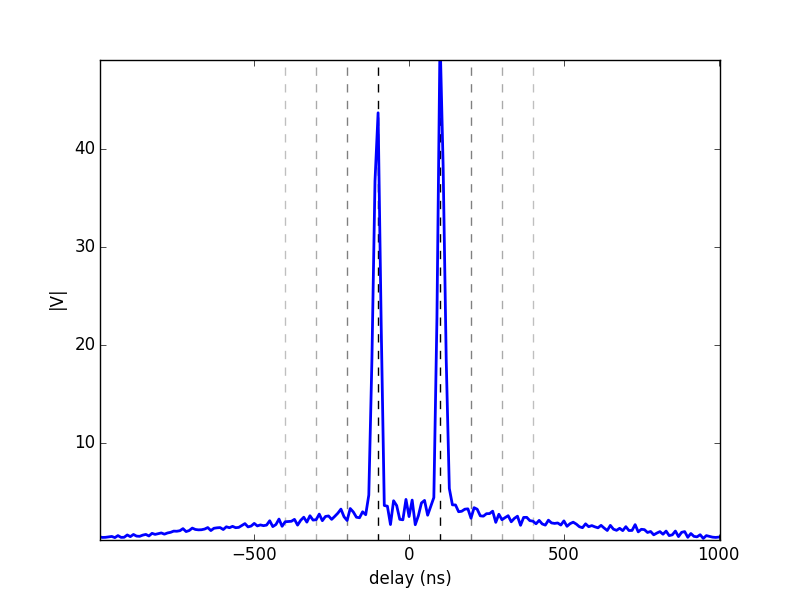
\includegraphics[width=0.4\textwidth]{6250_yy_xtalk_that_night_BLtype1_median_d.png}
\caption{\textit{Left}: The delay transform of the average signal for the night for all 30\,m baselines in the array. \textit{Right}: The average of these signals. The dotted lines show the light-travel-time between increasing grid separations (1, 2, 3 and 4-unit 30\,m baselines). There is a clear pile-up of signal at 1-unit delays.}
\label{fig:xtalk-for-BL1}
\end{figure}

\begin{figure}
\centering
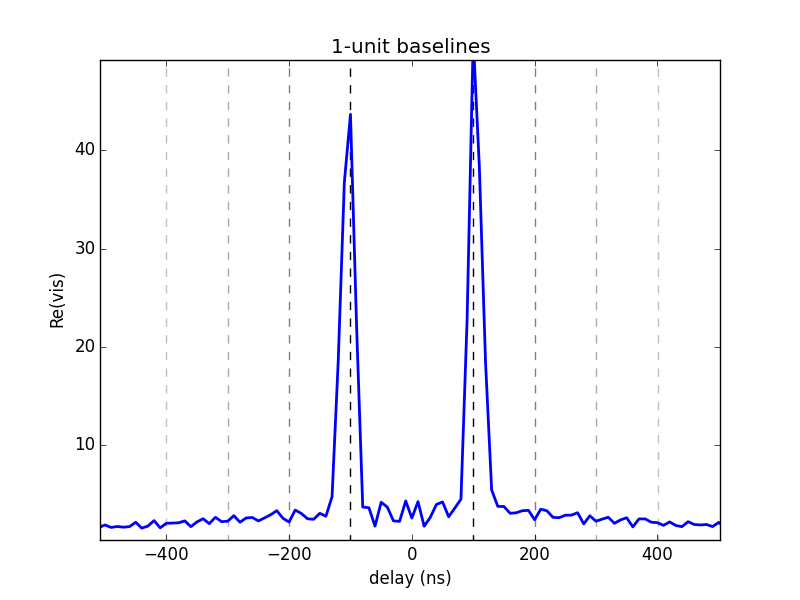
\includegraphics[width=0.4\textwidth]{xx_1unit_xtalk_d.png}
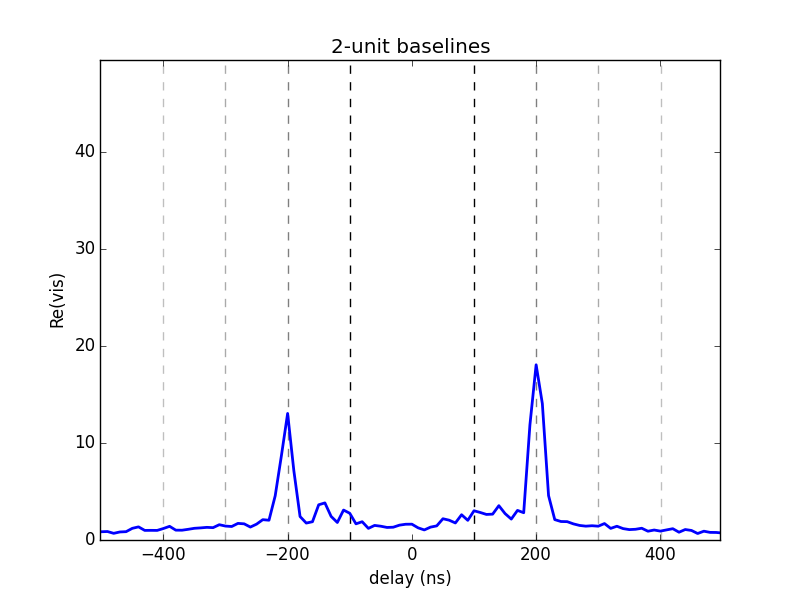
\includegraphics[width=0.4\textwidth]{xx_2unit_xtalk_d.png}
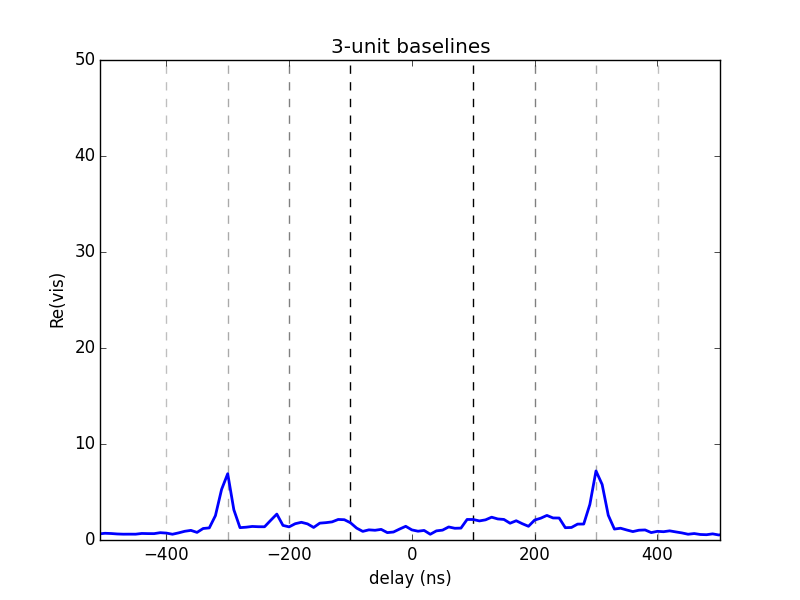
\includegraphics[width=0.4\textwidth]{xx_3unit_xtalk_d.png}
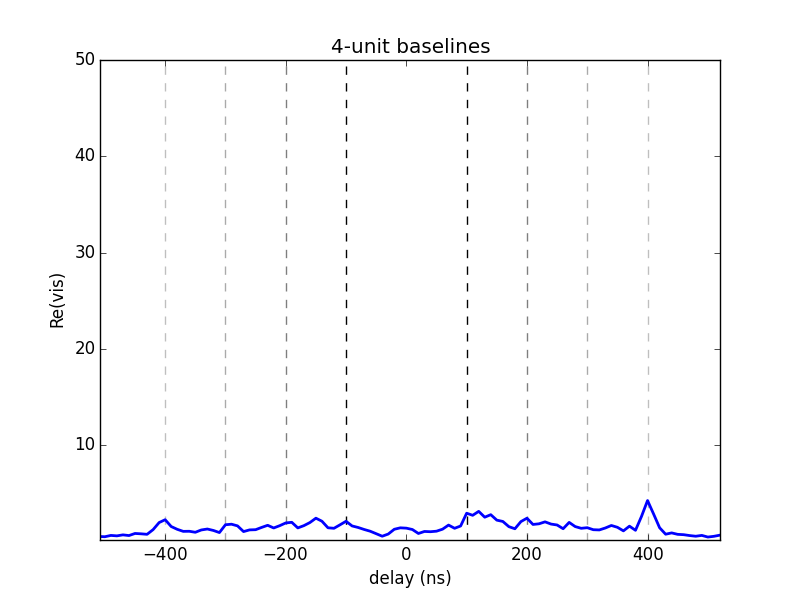
\includegraphics[width=0.4\textwidth]{xx_4unit_xtalk_d.png}
\caption{The average signal over the night in delay-space, averaged for baseline types of 30, 60, 90 and 120\,m separations.}
\label{fig:the-money-plot}
\end{figure}

XXX R-SQUARED PLOT\\
XXX RIDHIMA PLOTS: PICTOR FIELD BEFORE AND AFTER D TERMS ON COMMON FLUX SCALE\\

\section{Why we need to care}

Reasons for implementing accurate crosstalk subtraction:
\begin{itemize}
\item Most of the crosstalk power lies outside of the horizon, especially on the shortest baselines, limiting our ability to probe the EoR window.
\item Inaccurate crosstalk subtraction leaves artefacts in images (XXX NEED FIGURE) which will throw a spanner in the works for imaging-based calibration such as FHD.
\item Without any accounting for crosstalk, the $XY$ and $YX$ visibilities are completely overpowered by crosstalk coupled to $XX$ and $YY$ correlations, limiting our ability to constrain astrophysical polarization as a separate contaminant of the EoR window.
\end{itemize}

\bibliographystyle{plain}
\bibliography{xtalkmemoBib}

\end{document}